\section{git}
\begin{frame}{git}
  \begin{center}
    \includegraphics[width=100px]{../Notes/img/git.pdf}
  \end{center}
  \tableofcontents[sectionstyle=show/hide,
                   subsectionstyle=show/show/hide,
                   subsubsectionstyle=show/show/show]
\end{frame}

\subsection{Warum?}
\begin{frame}{Warum?}
  \begin{block}{Warum Versionskontrolle?}
    \begin{itemize}
      \item Backup
      \item vereinfachte Kollaboration
      \item Protokollierung
    \end{itemize}
  \end{block}
  \begin{block}{Warum Git?}
    \begin{itemize}
      \item \textit{distributed} Version Control System
      \item sehr schnell
      \item setzt sich momentan durch
    \end{itemize}
  \end{block}
\end{frame}

\begin{frame}{Übersicht}
  \begin{center}
    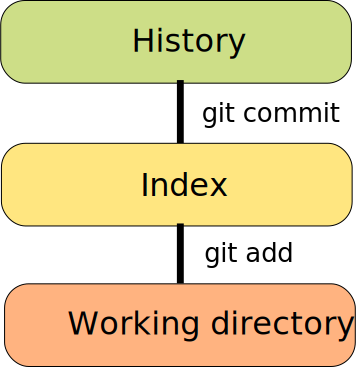
\includegraphics[width=150px]{img/git_repo.pdf}
  \end{center}
\end{frame}

\begin{frame}{Übersicht}
  \begin{center}
    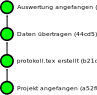
\includegraphics[width=150px]{../Notes/img/commits.pdf}
  \end{center}
\end{frame}

\subsection{Befehle}
\begin{frame}{Repository erstellen}
  \begin{tabular}{lp{20em}}
    \texttt{git init} & Erzeugt ein leeres Repository im jetzigen Ordner \\
    \texttt{git clone [\textit{url}]} & Kopiert ein Repository aus dem Internet
  \end{tabular}
\end{frame}

\begin{frame}{Informationen abrufen}
  \begin{tabular}{lp{20em}}
    \texttt{git status} & Zeigt an, welche Dateien geändert wurden und welche bereits im Index sind \\
    \texttt{git log}    & Zeigt alle gespeicherten Commits an
  \end{tabular}
\end{frame}

\begin{frame}{Dateien zum Index hinzufügen}
  \begin{tabular}{lp{20em}}
    \texttt{git add} & Fügt eine Datei oder einen Ordner (mit Inhalt) zum Index hinzu \\
    \texttt{git rm [-r]}  & Löscht eine Datei aus dem Ordner und schreibt die Löschung in den Index  \\
    \texttt{git mv}  & Genauso, aber die Datei wird verschoben
  \end{tabular}
\end{frame}

\begin{frame}{Commits erstellen}
  \begin{tabular}{lp{20em}}
    \texttt{git commit} & Speichert die Änderungen im Index als Commit ab
  \end{tabular}
\end{frame}

\begin{frame}{Änderungen runter-/hochladen}
  \begin{tabular}{lp{20em}}
    \texttt{git pull} & Neue Commits runterladen \newline
                      Falls man noch neue lokale Commits hat führt git einen \textit{merge} durch \\
    \texttt{git push} & Neue Commits hochladen \newline
                      Geht nur, wenn keine neuen Commits im zentralen Repository sind \newline
                      Wenn ja, erst einmal \texttt{git pull} verwenden
  \end{tabular}
\end{frame}

\begin{frame}{Manuell mergen}
  \begin{tabular}{lp{20em}}
    \texttt{git mergetool} & Startet ein Programm, mit dem man manuell mergen kann, falls die Automatik nicht funktioniert
  \end{tabular}
\end{frame}

\subsection{Hoster}
\begin{frame}{Hoster}
  \begin{itemize}
    \item $
      \begin{array}{l}
        \includegraphics[height=18px]{../Notes/img/octocat.jpg}
      \end{array} $ \textbf{Github} (\url{https://github.com/})\\
      kostenlose öffentliche Repositories, gute UI
    \item $
      \begin{array}{l}
        \includegraphics[height=18px]{../Notes/img/bitbucket.png}
      \end{array} $ \textbf{Bitbucket} (\url{https://bitbucket.org})\\
      kostenlose private Repositories
  \end{itemize}
\end{frame}

